\newpage
\begin{center}
	\huge{Kryptologie}
\end{center}
%TODO 2 Teile im Pdf?
\section{Grundbegriffe und einfache Verfahren}
	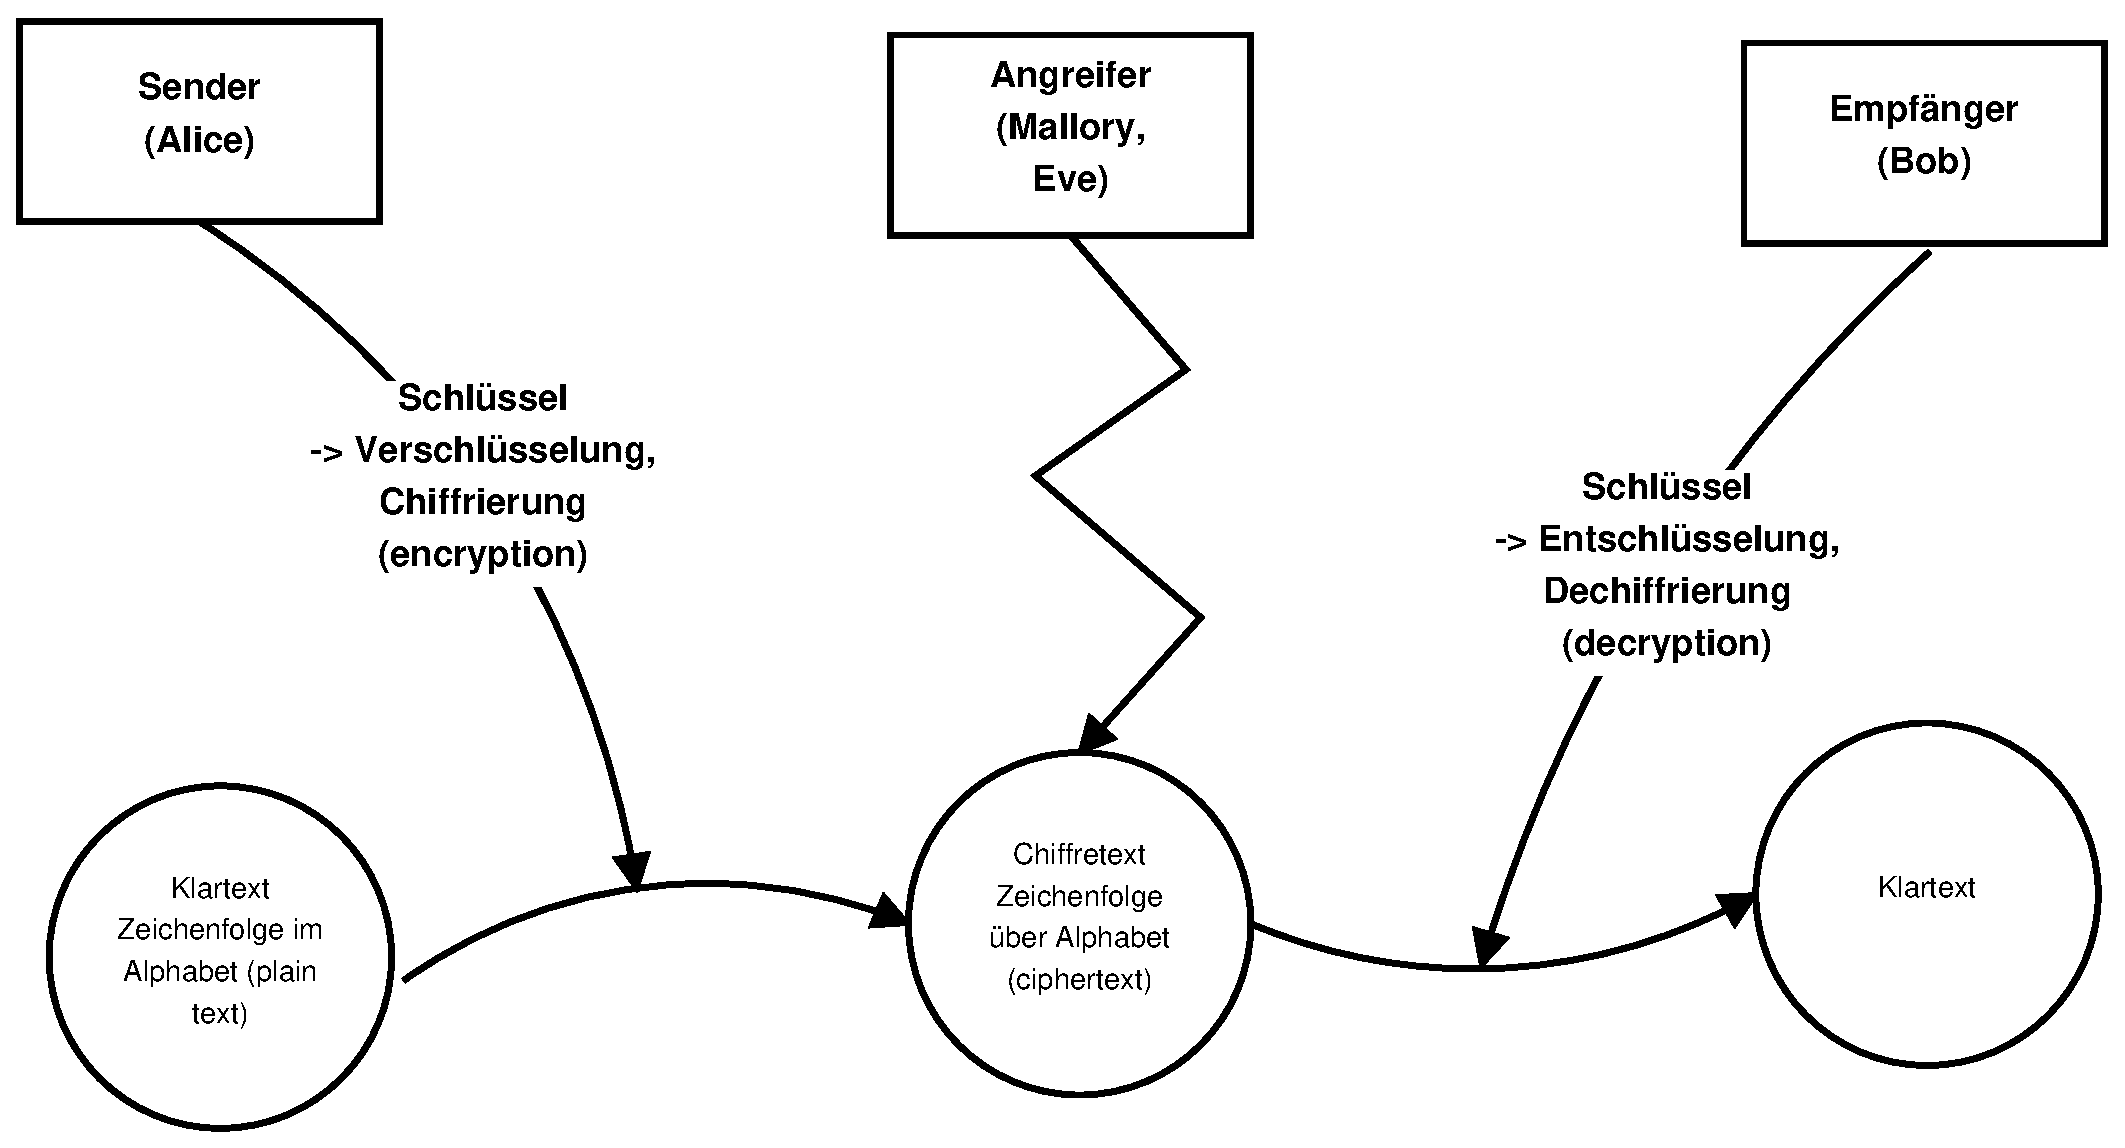
\includegraphics[width=\textwidth]{eps/pic01.eps}

	\textbf{Verschlüsselung erfordert}
	\begin{itemize}
		\item Verschlüsselungsverfahren, Chiffrieralgorithmus (Funktion $E$)
		\item Schlüssel $k_e$ (encryption key)
	\end{itemize}
	$E(\underset{\mbox{\scriptsize Klartext}}{m},\underset{\mbox{\scriptsize Schlüssel}}{k_e})=\underset{\mbox{\scriptsize Chiffretext}}{C}$ \\
	$k_e$ stammt aus der Menge $\mathcal{K}$ von Schlüsseln.\\
	Für ein festes $k_e$ muss $E\lrr{.,k_e}$ injektiv sein, das heißt\\
	$m_1\neq m_2 \Rightarrow E\lrr{m_1,k_e}\neq E\lrr{m_2,k_e}$
	
	\textbf{Entschlüsselung erfordert}
	\begin{itemize}
		\item Entschlüsselungsalgorithmus, Dechiffrierverfahren (Funktion $D$)
		\item Einen von $k_e$ abhängigen Decryption-Key $k_d$
	\end{itemize}
	$D(c,k_d)=m\quad D\lrr{.,k_d}=E\lrr{.,k_e}^{-1}$
	\subsection{Symmetrisches \& Asymmetrisches Verschlüsselungsverfahren}
		Ist $k_d=k_e$, oder falls $k_d$ leicht aus $k_e$ berechenbar ist, so spricht man von einem \textbf{symmetrischen Verschlüsselungsverfahren}.\\
		Lässt sich $k_d$ aus $k_e$ nur mit unverhältnismäßig großem Aufwand berechnen, so kann man $k_e$ öffentlich machen. Das heißt \textbf{Public Key Verfahren} oder auch \textbf{asymmetrisches VerschlÜsselungsverfahren}. (Kein Schlüsselaustausch notwendig!)
	
		In einem symmetrischen Verfahren werden $\binom{n}{2}=\dfrac{n\lrr{n-1}}{2}$ Schlüssel benötigt, wenn $n$ die Anzahl aller Verbindungspaare ist. Bei einem assymmetrischen Verfahren werden lediglich $2n$ Schlüssel benötigt.
	\subsection{Beispiel}
		\subExBegin{a)}
			\item $R=S=\lrc{0,\dots,25}$ \\
				Verfahren - \textbf{Verschiebechiffre}\\
				$\mathcal{K}=\lrc{0,\dots,25}$ \\
				Wähle Schlüssel $i\in\mathcal{K}$\\
				$x\in R$ Verschlüssle $x\rightarrow x+i\mod 26$\\
				$m=x_1\dots x_r\quad x_i\in R$\\
				$E\lrr{m,i}=\underbrace{\lrr{\lrr{x_1+i}\mod 26}}_{y_1}\dots\underbrace{\lrr{\lrr{x_r+i}\mod 26}}_{y_r}=c$\\
				Entschlüssle $y\in R \rightarrow y-i\mod 26$\\
				$D\lrr{c,i}=\lrr{\lrr{y_1-i}\mod 26}\dots\lrr{\lrr{y_r-i}\mod 26}=m$
			\item Verallgemeinerung: \textbf{Zeichenweise Substitutionschiffren}\\
				$R=S=\lrc{0,\dots,25} \quad\mathcal{K}=$ Menge der Permutationen von $R$\\
				Wähle $\pi\in\mathcal{K}$\\
				$m=x_1\dots x_r\quad x_i\in R$\\
				$E\lrr{m,\pi}=\underbrace{\pi\lrr{x_i}}_{y_1}\dots\underbrace{\pi\lrr{x_r}}_{y_r}=c$\\
				$c=y_1\dots y_r$\\
				$D\lrr{c,\pi^{-1}}=\pi^{-1}\lrr{y_1}\dots\pi^{-1}\lrr{y_r}=m$\\
				Jetzt ist $\lrabs{\mathcal{K}}=26!\equiv 4\cdot10^{26}$
			
				Angenommen ein Angreifer kann $10^{12}$ Schlüssel in der Sekunde testen.\\
				Angenommen $50\%$ der Schlüssel getestet werden um den richtigen zu finden.\\
				Dann werden $2\cdot 10^{14}$ Sekunden, also ungefähr $6.000.000$ Jahre benötigt.
		\subExEnd
	\subsection{Bemerkung}
		Das Verfahren aus 1.3b) ist bei Verschlüsselung von natürlichsprachlichen Texten völlig unsicher. Das liegt an der charakteristischen Buchstabenhäufigkeitsverteilung.
	\subsection{Prinzip von Kerkhoffs (1835-1903)}
		Die Sicherheit einer Verschlüsselung darf nicht von der Geheimhaltung des Verfahrens abhängen, sondern nur von der Geheimhaltung des Entschlüsselungsschlüssels $k_d$.
	\subsection{Kryptoanalyse}
		\begin{itemize}
			\item Ciphertext-Only-Angriff
			\item Known-Plaintext-Angriff
			\item Chosen-Plaintext-Angriff
			\item Chosen-Ciphertext-Angriff
	\end{itemize}
\section{One-Time-Pad und perfekte Sicherheit}
	\subsection{Lauftextverschlüsselungen}
		Klartext(über $R=\lrc{0,\dots,25}$) Wähle \textit{Schlüsseltext} der gleichen Länge über $R$\\
		Addiere Schlüsseltext zeichenweise zu Klartext $\mod 26$,
		
		\textbf{Beispiel}
		
		\begin{tabular}{lcccccccccc}
			Klartext&P&E&T&E&R&15&4&19&4&17\\
			Schlüsseltext&H&A&U&C&K&7&0&20&2&10\\\cline{7-11}
			&&&&&&22&4&13&6&1\\
			&&&&&&W&E&N&G&B
		\end{tabular}
		
		Das nennt sich \textbf{kontextabhängiges Verschlüsselungsverfahren}.
	\subsection{One-Time-Pad}
		Klartextalphabet $R=\lrc{0,1}=\mz_2$\\
		Klartext $m$ hat die Länge $n$ über $\mz_2$\\
		Wähle als Schlüsselfolge eine Zufallsfolge $k$ der Länge $n$ und addiere bitweise $\mod 2$ (XOR).\\
		$c=m\oplus k$
		
		\textbf{One-Time-Pad}: Schlüssel nur einmal verwenden.\\
		$c_1=m_1\oplus k$\\
		$c_2=m_2\oplus k$\\
		Angreifer fängt $c_1$ und $c_2$ ab:\\
		$c_1\oplus c_2 = m_1\oplus k\oplus m_2\oplus k=m_1\oplus m_2$\\
		Wenn $m_1,m_2$ sinnvolle Texte sind, so gibt es in $m_1\oplus m_2$ statistische Auffälligkeiten $\Rightarrow$ Angriffsmöglichkeiten.
		
		\begin{tabular}{lcccc}
		Klartext&$m_1$&$m_2$&\dots &$m_n$\\
		Schlüsselfolge&$S_1$&$S_2$&\dots &$S_n$\\
		$m_1\oplus S_1$&$m_2\oplus S_2$&\dots &$m_n\oplus S_n$
		\end{tabular}
		
	\subsection{Zufallsfolge der Länge \texorpdfstring{$n$}{n}}
		Erzeugt durch binäre symmetrische Quelle mit Wahrscheinlichkeit $50\%$ 0 oder 1, unabhängig von den schon erzeugten Bits. Also hat jede binäre Folge die Auftrittswahrscheinlichkeit $\dfrac{1}{2^n}$.
		
	\subsection{One- Time Pad ist unter den Voraussetzungen von 2.3/2.2 perfekt sicher}
		Das heißt für jeden Klartext $m$ und jeden denkbaren Chiffretext $c$ gilt:
		\[pr(m|c)=pr(m)\]
		$pr(m|c)$: a- priori Wahrscheinlichkeit für $m$, falls $c$ empfangen wurde.\\
		$pr(m)$: a- priori Wahrscheinlichkeit für $m$
		
		Warum ist One- Time- pad perfekt sicher?\\
		Formaler Beweis: Bayer'sche Formel\\
		Intuitiv: $m$ fester Klartext. $m\in\mz_2^n$\\
		Jeder Schlüssel $k\in\mz_2^n$ ist gleicher.\\
		$m\oplus k$ sind gleich wahrscheinlich, wenn $k$ über alle möglichen Schlüssel läuft.

\section{Symmetrische Blockchiffren}
	Blockchiffren $\underset{\mbox{\scriptsize Blöcke der Länge }n>1}{|\underbrace{\dots}|\underbrace{\dots}|\underbrace{\dots}|}$\quad Klartext
	
	Jeder Block wird einzeln verschlüsselt. Gleiche Blöcke werden gleich verschlüsselt (Es gibt aber auch andere Betriebsverschlüsselungen.\\
	$R=S=\mz_2$. Wie viele Blockchiffren der Länge $n$ gibt es?\\
	$\fbox{0...0}\fbox{0...01}\dots\dots\dots\fbox{1...1}$ $2^n$ Blöcke der Länge $n$\\
	Jeder dieser Blöcke wird in einen anderen umgewandelt\\
	Jeder Blockchiffre entspricht Permutation der $2^n$ Blöcke (Länge $n$) über $\mz_2$.\\
	Wenn alle Permutationen als Schlüssel zugelassen sind, so hat Schlüsselraum die Größe $\lrr{2^n}!$\\
Speicherbedarf für einen Schlüssel: $\underbrace{|*...*|*...*|\dots\dots\dots|*...*|}_{2^n\mbox{\scriptsize Blöcke mit }n\mbox{\scriptsize\ Bit}}$\\
	$n\cdot 2^n$ Bit, z.B. $n=64$\\
	Speicherung eines Schlüssels: $2^6\cdot 2^64=135\mbox{ TB}$
	
	\subsection{Lineare Blockchiffren}
		Klartextalphabet = Chiffretextalphabet = $\mz_k=\lrc{0,...,k-1}$\\
		Blocklänge $n$: Block $\in\mz^n$\\
		Block $m=(V_1,...,V_n)$, $V_i\in\mz_k$\\
		Schlüssel: $n\times n$- Matrix $A$ mit Einträgen in $\mz_k$ (und zusätzlicher Bedingung)\\
		Verschlüsselung: $c=m\cdot A=(w_1,...,w_n)$\\
		$\mz_5,n=2:\ (3,4)\cdot\lrv{1&2\\3&4}=\lrv{0&2}$\\
		$a\oplus b=a+b\mod k$\\
		Jedes Chiffrezeichen hängt von allen Klartextzeichen innerhalb eines Blocks ab\\(\textbf{Diffusion}).\\
		Wann ist diese Abbldung $m\in\mz_k^n\mapsto m\cdot A\in\mz_k^n$ injektiv, d.h. eine Permutation auf $\mz_k^n$?\\
		Genau dann, wenn $A$ invertierbar ist, d.h. $A^{-1}\ n\times n$- Matrix über $\mz_k$ mit der Eigenschaft $A^{-1}\cdot A=A\cdot A^{-1}=E_n=\begin{pmatrix}1&\dots&0\\\vdots&1&\vdots\\0&\dots&1\end{pmatrix}$\\
		Entschlüsseln: $c\cdot A^{-1}=(mA)\cdot A^{-1}=m(A\cdot A^{-1})=m\cdot E_n=m$
		
		$A\ n\times n$- Matrix über $\mz_k$, $\det(A)\in\mz_k$\\
		$2\times 2$- Matrix $\det\lrv{a&b\\c&d}a\cdot d-b\cdot c$\\
		$\mz_5:\ A=\lrv{1&2\\3&4}\quad\det(A)=(1\cdot 4-2\cdot 3)\mod 5=3$.
		
		$A$ invertierbar $\Leftrightarrow$ $\det(A)$ invertierbar in $\mz_k$ bezüglich $\odot$ $\Leftrightarrow\ \ggT(\det(A),k)=1$.\\
		$A^{-1}=(\det(A))^{-1}\cdot B$, $B=(b_{ij}),\ b_{ij}=(-1)^{i+j}\det(A_{ij})$\\
		$A_{ji}$ entsteht aus $A$ durch Streichen der $j$- ten Zeile und $i$- ten Spalte.\\
		Speziell $n=2$: $A=\lrv{a&b\\c&d}$, $\det(A)=ad-bc$\\
		$A^{-1}=\det(A)^{-1}\lrv{d&-b\\-c&a}$
		
		\textbf{Bsp.:} $\mz_6$, $A=\lrv{0&1\\1&3}$, $\det(A)=-1\mod 6=5$ $\ggT(5,6)=1$\\
		$5^{-1}=5$, da $5\odot 5=1$\\
		$A^{-1}=5^{-1}\lrv{3&-1\\-1&0}=\lrv{3&1\\1&0}$ über $\mz_6$.
		
		$m=(1,3)$\\
		Verschlüsselung: $m\cdot A=(1,3)\lrv{0&1\\1&3}=(3,4)=c\mod 6$\\
		Entschlüsselung: $c\cdot A^{-1}=(3,4)\lrv{3&1\\1&0}=(1, 3)=m$\\
		Schlüssel: $A$\\
		$\mz_2$: $n^2$ Bit.\\
		$n=64$. Wie viele invertierbare Matritzen $(64\times 64)$ über $\mz_8$ gibt es?\\
		$(2^{64}-1)(2^{64}-2)\dots(2^{64}-2^{63})\approx 0,29\cdot 2^{4061}$\\
		(Groß, aber winzig im Vergleich zu $\lrr{2^{64}}!\approx 2^{10^{21}}$)
		
		Blockchiffren über $\mz_k$, Blocklänge $n$.\\
		$m\in\lrr{\mz_k}^n$, Schlüssel $A$ $n\times n$-Matrix über $\mz_k$ $m\rightarrow mA=c$.\\
		$A$ invertierbar $\Leftrightarrow \ggT(\det(A), k)=1$\\
		$\det\lrv{a&b\\c&d}=a\cdot b-b\cdot c$
	\subsection{Known-Plaintext-Angriff auf lineare Chiffren}
		Benötigt $n \underset{m_1,\dots,m_n}{\mbox{Klartextblöcke}}$ und zugehörige $\underset{c_1,\dots,c_n}{\mbox{Chiffretextblöcke}}$\\
		$m_iA=c_i$\\
		$A$ ist unbekannt. Möglich, falls die Matrix $M=\lrv{m_1\\\vdots\\m_n}$ invertierbar ist.\\
		(Sicherstellbar bei Chosen-Plaintext-Angriff)\\
		Setze $C=\lrv{c_1\\\vdots\\c_n}$. Dann gilt $M\cdot A=C$\\
		Der Angreifer berechnet $M^{-1}$. $M^{-1}\cdot C = M^{-1}\lrr{MA}=E_n\cdot A = A$
		
		\textbf{Beispiel}
		
		$n=2\quad k=26$\\
		Angenommen wir wissen: KRYPTO ist mit einer linearen Chiffre $\lrr{n=2,\mz_{26}}$ in QLIPRL verschlüsselt worden.
		
		\begin{tabular}{rr|rr|rr}
			K&R&Y&P&T&O\\
			10&17&24&15&19&14\\
			\multicolumn{2}{c|}{$m_1$}&\multicolumn{2}{c|}{$m_2$}&\multicolumn{2}{c}{$m_3$}
		\end{tabular}
		$\qquad \rightarrow\qquad$
		\begin{tabular}{rr|rr|rr}
			Q&L&I&P&R&L\\
			16&11&8&15&17&11\\
			\multicolumn{2}{c|}{$c_1$}&\multicolumn{2}{c|}{$c_2$}&\multicolumn{2}{c}{$c_3$}
		\end{tabular}
		
		$\underset{2|\det M, 2|26}{M = \lrv{m_1\\m_2}=\lrv{10&17\\24&15}}$ funktioniert nicht.\\
		$M=\lrv{m_1\\m_3}=\lrv{10&17\\19&14}$\\
		$\det M = 10\cdot 14 - 17\cdot 10 \mod 26 = 25\quad\rightarrow$ teilerfremd zu $26$.
		
		$\lrr{\det M}^{-1} = 25\lrr{=-1\mod 26}$\\
		$M^{-1} = -\lrv{14&-17\\-19&10} = \lrv{-14&17\\19\\-10}=\lrv{12&17&19&16}$\\
		$C=\lrv{c_1\\c_3}=\lrv{16&11\\17&11}$\\
		$A=M^{-1}\cdot C = \lrv{12&17\\19&16}\cdot\lrv{16&11\\17&11}=\lrv{481&319\\576&385}=\underset{\mod 26}{\lrv{13&7\\4&21}}$
		
		Test:\\
		$\lrv{10&17}\cdot\lrv{13&7\\4&21}=\lrv{198&427}=\lrr{16,11}$\\
		$\lrv{24&15}\cdot\lrv{13&7\\4&21}=\lrv{372&483}=\lrr{8,15}$\\
		$\lrv{19&14}\cdot\lrv{13&7\\4&21}=\lrr{17,11}$
	\subsection{Bemerkung}
		Häufig werden zur Erhöhung der Sicherheit mehrere Blockchiffrierungen hintereinander aungewendet.\\
		Das ist nicht immer sinnvoll:\\
		z.B.: $2$ lineare Chiffren mit $2$ Schlüsseln $A_1,A_2$ hintereinander ausführen.\\
		$m\rightarrow\underbrace{\lrr{A_2A_1}}_{n\times n} m \quad \rightarrow\quad$ Chiffretext vom selben Typ. (Mit Matrix $A_2,A_1$)
\section{Der Advanced Encryption Standard (AES)}
	Anfang der 1970'er Jahre: DES Blocklänge $64$ Bit mit Schlüssellänge $56$ Bit\\
	Ab 1990'er Jahre war Brute-Force möglich.\\
	NIST öffentliche Ausschreibung $\rightarrow$	2000 Rijndael-Verfahren (J.Daemen, V.Rijmen) $\rightarrow$ AES\\
	2002: FIPS 197
	\subsection{Struktur des AES}
		AES ist eine iterierte Blockchiffre\\
		Blocklänge $\underline{128},192,256$ Bit\\
		Schlüssell. $\underline{128},192,256$ Bit\\
		$\underline{10},12,14$ Runden\\
		Zwischenergebnisse werden Zustände (states) genannt.
		
		Jede Runde (bis auf 10.) besteht aus 3 Transfusionen und Rundenschlüsseladdition
		%TODO: Bild
		Klar- und Chiffretextblöcke und States werden beschreieben durch $4\times 4$ - Matrizen.\\
		$a_ij$ Bytes $\lrv{a_{00}&\dots&a_{03}\\\vdots&&\vdots\\a_{30}&\dots&a_{33}}\hat{=} 128$ Bit $\hat{=} a_{00}a_{10}a_{20}a_{30}a_{01}a_{11}$\\
		Gelegentlich werden Bytes als Elemente in einem Körper der Ordnung $2^8$ $\mathbb{F}_{2^8}$ aufgefasst.
	\subsection{Der Körper \texorpdfstring{$\mathbf{\mathbb{F}_{2^8}}$}{F}}
		$\mathbb{F}_{2^8}$ = Menge aller Polynome über $\mz_2$ vom Grad $<8$\\
		$\lrr{b_7,b_6,b_5,\dots,b_0}\leftrightarrow b_7x^7+b_6x^6+\dots+b_1x+b_0$\\
		Addition: koffizientenweise in $\mz_2$\\
		Multiplikation: Multiplikation normal, reduziere $\mod$ \textbf{irreduzieble} Polynome vom Grad $8$.\\
		irreduziebles Polynom $x^8+x^4+x^3+x+1$\\
		$\lrr{10000011}\odot\lrr{00001010}$\\
		$x^7+x+1\odot x^3+x$\\
		$\lrr{x^7+x+1}\cdot\lrr{x^3+x}=x^{10}+x^4+x^3+x^8+x^2+x$ reduziert $\mod h$ \\
		$x^{10}+x^8+x^4+x^3+x^2+x : x^8+x^4+x^3+x+1=x^2$\\
		$-\lrr{x^{10}+x^6+x^5+x^3+x^2}$\\
		$x^8+x^6+x^5+x^4+x$\\
		$-\lrr{x^8+x^4+x^3+x+1}$\\
		$x^6+x^5+x^3+1 =\lrr{x^7+x+1}\odot\lrr{x^3+x}$\\
		$\lrr{01101001}$
		
		$g\neq 0$\\
		$g\odot g^{-1} =1$\\
		$s\cdot g + t\cdot h=1$\\
		$s\mod h = g^{-1}$
		
		In $\mz_2\lra{x}$ gilt der Erweiterte Euklidische Algorithmus.\\
		$f,g\neq 0$ Bestimme $u,v\in\mz_2\lra{x}:\ggT\lrr{f,g}=u\cdot f+v\cdot g$\\
		$f\in\mathcal{F}_{2^8}\quad f^{-1}$ bezüglich $\odot$\\
		$1=\ggT(f,\underbrace{h}_{\mbox{\scriptsize irred.}}) = u\cdot h+v\cdot f$\\
		$1=\lrr{u\cdot h+v\cdot f}\mod h=\lrr{v\cdot f}\mod h=\lrr{\lrr{v\mod h}\cdot f}\mod h$
		
		\textbf{(Verkürzter) erweiterter Euklidischer Algorithmus in }$\mathbf{\mz_2\lra{x}}$
		
		Sei $f,g\in \mz_2\lra{x}\quad g\neq 0\quad \grad\lrr{f}\geq\grad\lrr{g}$\\
		Bestimme $v\in\mz_2\lra{x}$ mit $v\cdot g\equiv\ggT\lrr{f,g}\;\;\lrr{\mod f}$
		\subExBegin{(1)}
			\item Setze $s(x)=f(x),t(x)=g(x)$\\
				$v_1(x)=0,v_2(x)=1,v(x)=1$
			\item Solange $s(x)\mod t(x)\neq 0$ wiederhole:\\
				$q(x) =s(x)\div t(x), r(x)=s(x)\mod t(x)$\\
				$v(x)=v_1(x)-q(x)\cdot v_2(x)$\\
				$v_1(x)=v_2(x)\quad v_2(x)=v(x)\quad s(x)=t(x)\quad t(x)=r(x)$
			\item Ausgabe: $t(x) =\ggT\lrr{f,g}$\\
				$v(x)=v\cdot g$
		\subExEnd
		Es gilt $\lrr{g+f}^{-1}\neq g^{-1}+f^{-1}$
	\subsection{SubBytes-Transformation}
		(Sub für Substitution)\\
		Eingabe: Zustand $S_i=\lrv{b_{00}&\dots&b_{03}\\\vdots&&\vdots\\b_{30}&\dots&b_{33}}\quad b_{ij}$ Bytes.\\
		Jedes Byte wird einzeln verschlüsselt.\\
		$g=\lrr{b_7,b_6,\dots,b_0}$ Byte
		\subExBegin{(1)}
			\item Fasse $g$ als Element in $\mathbb{F}_{2^8}$ auf.\\
				Falls $g\neq 0$ ist, bilde $g^{-1}$\\
				Falls $g=0$ ist, so lasse $g$ unverändert.
			\item Ergebnis $\lrr{C_7,C_6,\dots,C_0}$ wird affin-linear abgebildet.\\
				$\lrr{c_0c_1\dots c_7} A+B=\lrr{d_0\dots d_7}$\\
				Das Ergebnis von SubBytes ist $\lrr{d_7d_6\dots d_0}$.\\
				Dabei gilt $A=\lrv{11111000\\\vdots}$\\
				(übrige Zeilen entstehen durch zyklische Shifts um $1-7$ Stellen)\\
				$b=\lrr{11000110}$
		\subExEnd
		In AES wird SubBytes durch Tablelookup realisiert:\\
		$16\times 16$-Matrix, Einträge sind $0,\dots,255$ binär codiert $\leftrightarrow$ Bytes\\
		Input: $\lrr{b_7b_6\dots b_0}\qquad b_7b_6b_5b_4\rightarrow$ bestimmt Zeile $x$, $b_3b_2b_1b_0\rightarrow$ bestimmt Spalte $y$ der Matrix\\
		An der Stelle $\lrr{x,y}$ steht das Ergebnis.
	\subsection{Shift Rows und Mix Columns Transfer}
		\begin{itemize}
			\item \textbf{Shift Rows}
			
				Jede der $4$ Zeilen der $4\times 4$-Matrix (nach SubBytes) wird zyklisch nach links verschoben.\\
				$i$-te Zeile um $\lrr{i-1}$-Stellen, wobei $i\in\lrc{1,2,3,4}$\\
				$\lrv{b_{00}&\dots&b_{03}\\b_{10}&\dots&b_{13}\\\vdots&\vdots&\vdots}\rightarrow\lrv{b_{00}&\dots&\dots&b_{03}\\b_{11}&b_{12}&b_{13}&b_{10}}$
			\item \textbf{Mix Columns}
			
				Jedes Byte in der $4\times 4$-Input-Matrix wird als Element des $\mathbb{F}_{2^8}$ aufgefasst. \\
				Multipliziere diese $4\times 4$-Matrix von links $M=\lrv{x&x+1&1&1\\1&x&x+1&1\\1&1&x&x+1\\x+1&1&1&x}$\\
				$M\cdot\lrv{p_{00}&\\p_{10}&x\times x\\p_{20}&\\p_{30}&} = \lrv{xp_{00}+xp_{10}+p_{10}+p_{20}+p_{30}\\p_{00}+xp_{10}+xp_{20}+p_{20}+p_{30}}$\\
				Dabei ist $\cdot$ in der Regel $\odot$ in $\mathbb{F}_{2^8}$
		\end{itemize}
		Verwendet werden diese Verfahren für \textbf{Diffusion} und \textbf{Konfusion}
	\subsection{Rundenschlüsselerzeugung}
		Ausgangsschlüssel $128$ Bit. Schreibe als $4\times 4$-Matrix von Bytes, spaltenweise.\\
		$w(0),w(1),w(2),w(3)$ Spalten \\
		Definiere $40$ weitere Spalten à $4$ Bytes.\\
		Angenommen $w(0),\dots,w(i-1)$ sind schon definiert $\lrr{i\geq 4}$
		\begin{itemize}
			\item $i\not\equiv 0\lrr{\mod 4}$:\\
				$w(i)=w\lrr{i-1}\oplus w\lrr{i-4}$
			\item $i\equiv 0\lrr{\mod 4}$:\\
				$w(i)=T\lrr{w\lrr{i-1}}\oplus w\lrr{i-4}$
		\end{itemize}
		$T$ folgt Transformation $w\lrr{i-1}=\lrv{a\\b\\c\\d}$ mit $a,b,c,d$ Bytes.\\
		Wende Auf $\begin{array}{cccc}b&c&d&a\\e&f&g&h\end{array}$ SubBytes-Transformation an.\\
		Berechne $r\lrr{i}=(\underbrace{00000010}_{x})^{\frac{i-4}{4}}$ in $\mathbb{F}_{2^8}$\\
		$T\lrr{w\lrr{i-1}}=\lrv{e\oplus r(i)\\f\\g\\h}$ Rundenschlüssel $k_i$\\
		$\lrr{w\lrr{4i},w\lrr{4i+1},w\lrr{4i+2},w\lrr{4i+3}}$\\
		$i=0,1,\dots,10$
		
	\subsection{Entschlüsselung}
		Alle einzelnen Transformationen sind invertierbar. Kehre Algorithmus um und ersetztz alle Transformationen durch ihr Inverses.
		
	\subsection{Schnelligkeit und Sicherheit}
		\begin{itemize}
			\item Schnelligkeit:
			\begin{itemize}
				\item Software: $200\frac{\text{MBit}}{s}-2\frac{\text{GBit}}{s}$
				\item Hardware: $2\frac{\text{GBit}}{s}-70\frac{\text{GBit}}{s}$
			\end{itemize}
			\item Sicherheit
			\begin{itemize}
				\item Nach 2 Runden vollständige Diffusion
				\item Verfahren ist sicher gegen bekannte Angriffe (Differenzielle und lineare Kryptoanalyse)
			\end{itemize}
			\item Schlüsselerzeugungen mittels Subbytes soll verhindern, dass dbei Kenntnis von Teilen des Ausgangsschlüssels die übrigen Bits einfach zu ermitteln sind.
			\item Verschiedene Ausgangsschlüssel haben nie viele Rundenschlüssel gemeinsam.
		\end{itemize}
	
\section{Public- Key- Systeme}
	\subsection{Grundidee}
		Jeder Teilnehmer $A$ hat Paar von Schlüsseln
		\begin{itemize}
			\item Öffentlicher Schlüssel $P_A$
			\item Geheimer Schlüssel $G_A$
		\end{itemize}
		Zu jedem öffentlichen Schlüssel gibt es eine Verschlüsselungsfunktion	 $E_{P_A}=E(\circ, P_A)$ öffentlich bekannt.\\
		$B\overset{m}{\longrightarrow}A$\\
		$m\mapsto E_{P_A}(m)=c$
		
		\textbf{Bedingungen}
		\subExBegin{(1)}
			\item $m$ darf nicht mit realistischem Aufwand aus $E_{P_A}(m)$ berechenbar sein (natürlich muss $E_{P_A}(m)$ effizient berechenbar sein). $E_{P_A}$ ist eine \textbf{Einwegfunktion}.
			\item $A$ muss $m$ aus $c=E_{P_A}(m)$ effizient berechnen können mit Hilfe von $G_A$. $m=D_{G_A}(c)$\\
			Injektive Einwegfunktionen, die mit Zusatzinformation effizient invertierbar sind: \textbf{Geheimtürfunktionen} oder \textbf{trap door functions}.
			\item $G_A$ darf aus $P_A$ nicht effizient berechenbar sein.
		\subExEnd
		
		\textbf{Gibt es Einwegfunktionen?}\\
		Es gilt: $P\mpo NP$\\
		Notwendig: $P\neq NP$\\
		Es gibt einen Kandidaten für eine Einwegfunktion, auf denen geläufige Public- Key- Systeme basieren.
	
	\subsection{RSA- Verfahren}
		Rivest, Shamir, Adleman, 1977. Beruht auf Schwierigkeit zu faktorisieren
		\subExBegin{a)}
			\item Schlüsselerzeugung
				Man wähle zwei große Primzahlen $p,q$, $p\neq q$.
				\begin{itemize}
				\item $n=p\cdot q$\\
				Euler'sche $\varphi$ Funktion: $\varphi(n)=\mathcal{K}\in\mn:a\leq n, \ggT(a,n)=1$\\
				\item $\varphi(n)=(p-1)(q-1)$
				\item Wähle $e$ mit $\ggT(e,\varphi(n))=1$
				\end{itemize}
				
				\textbf{Öffentlicher Schlüssel} $P_a(n,e)$\\
				($p,q,\varphi(n)$ bleiben geheim)
				
				Wähle $1\leq d\leq\varphi(n)$ mit $e\cdot d\equiv 1(\mod \varphi(n))$ (Wie $\ggT(\varphi(n),e)=a\cdot e+b\cdot\varphi(n)$ für $a,b\in\mz$\\
				$a\cdot e\equiv\ggT(\varphi(n),e)\mod\varphi(n)$\\
				setze $d=a\mod\varphi(n)$
				
				\textbf{Gemeimer Schlüssel} $G_A=d$
			\item Verschlüsselung\\
				$B\overset{m'}{\longrightarrow} A$	\\
				$B$ codiert $m'$ als Zahl, zerlegt sie in Blöcke gleicher Länge, so dass jeder block eine Zahl $<n$ ist. Sei $m$ eine solche Zahl.\\
				$c=m^e\mod n$ Chiffretext
			\item Entschlüsselung\\
			$A$ bildet: $x^d\mod n$\\
			Behauptung: $c^d\mod n=m$\\
      Grund: Kleiner Satz von Fermat: Ist $r$ eine Primzahl, $a\in\mz$, für die
      $\ggT(p,a)=1$, do $a^{r-1}\equiv 1(\mod r)$\\
		$ed=1\mod(\varphi(n))$\\
		$e\cdot d=1+k\cdot\varphi(n)$ für $k\in\mz$\\
		$c^3=\lrr{m^e}^d=m^{ed}=m^{1+k\cdot\varphi(n)}=m^{1+(p-1)(q-1)\cdot k}=m\cdot\lrr{m^{(p-1)}}^{(q-1)\cdot k}\mod p$
		\begin{itemize}
			\item $p\not\|m$: $c^d=m(1)^{(q-1)\cdot k}=m\mod p$
			\item $p|m$: $c^d=m\cdot\lrr{m^{(p-1)}}^{(q-1)\cdot k}\equiv 0\ \mod p$\\
			$0\equiv m\mod p$\\
			$c^d\equiv m\mod p$
		\end{itemize}
		Ebenso für $q$\\
		$\Rightarrow c^d=m\mod q$\\
		$q|(c^d-m)$\\
		$p|(c^d-m)$\\
		$\Rightarrow\mbox{kgV}(p,q)|(c^d-m)$\\
		$pq|(c^d-m)$\\
		$c^d\equiv m\mod n$
		\subExEnd

	\subsection{Berechnung modularer Potenzen}
		Ziel: $m^e\mod n$ berechnen\\
		Problem: Overflow\\
		$e=\limsum{i=0}{k}e_i\cdot 2^i$\quad $e_k=1$ (Binärdarstellung von $e$)\\
		$m^e=m^{\limsum{i=0}{k}e_i2^i}=m^{e_k2^k}\cdot m^{e_{k-1}2^{k-1}}\cdot\dots\cdot m^{e_1\cdot 2}\cdot m^{e_0}$\\
		$=\lrr{\lrr{m^2\cdot m^{e_{k-1}}}^2\cdot m^{e^{k-2}}}^2\cdot)^2\cdot m^{e_1})^2\cdot m^{e_0}$

    \textbf{Beispiele für RSA:}\\
      1)\\
      $p=13,\ q=23$\\
      $n=p\cdot q=299$\\
      $\varphi(12\cdot 22)=264$\\
      kleinstmögliches $e=5$\\
      Öffentlicher Schlüssel $(n,e)=(299,5)$

      2) Bestimmung des geheimen Schlüssels: Entweder mit EEA $u,v\in\mz$
      bestimmen mit $u\cdot e+v\cdot\varphi(n)=1$. Dann $d=u\mod\varphi(n)$.

      In unserem Fall:\\
      $5|1\cdot 265+1=265$\\
      $d=\frac{265}{5}=53$\\
      Geheimer Schlüssel: $d=553$

      3) Verschlüsselung\\
      Klartext $m=212$\\
      $m^5\mod 299$ berechnen
      $212^2=44944\equiv 94(\mod 299)$\\
      $212^4\equiv 94^2=8836\equiv 165(\mod 299)$\\
      \dots

      4) Enschlüsselung\\
      Zu berechnen: $C^{53}\mod 299$\\
      \dots

      $n=pq$, $\varphi(n)=(p-1)(q-1), \ggT(e,\varphi(n))=1$\\
      $(n,e)$ öffentlich, $e\cdot d\equiv 1(\mod\varphi(n))$\\
      $d$ geheim.\\
      $m<n$. Verschlüsselung $c=m^e\mod n$\\
      Entschlüsselung $c^d\mod n=m$.

  \subsection{Sicherheit von RSA}
    \subExBegin{a)}
      \item Kein polynominialer Algorithmus zur Berechnung $e$- ter Wurzeln.
      \item Wie leicht ist die Bestimmung con $d$, falls $(e,n)$ bekannt.\\
        Leicht, falls $\varphi(n)$ bekannt ist (EEA)\\
        $\varphi(n)$ per Definition zu bestimmen, ist für große $n$ unmöglich.
        Leicht, falls $p.q$ bekann sind: $\varphi(n)=(p-1)(q-1)$. Gleich
        schwierig sind folgende Probleme:
        \begin{itemize}
          \item Bestimmung des geheimen Schlüssels
          \item Bestimmung von $\varphi(n)$\\
          \item Bestimmung des Faktorisierung von $n=p\cdot q$.
        \end{itemize}
      \item Komplexität der schnellsten Faktorisierungsalgorithmen:
        $O(e^{c\cdot(\log(n))^{1/3}(\log\log n)^{2/3}})$\\
        Faktorisierung von 768- Bit- Zahl: 2000 CPU- Jahre\\
        1024- Bit- Zahl: 1000 mal länger.\\
        Heutige Empfehlung: 2048 Bit. (ca $10^9$ mal länger als 1024- Bit-
        Zahl)\\
        3064 Bit RSQ $\Leftrightarrow$ AES 128 Bit
      \item Spielzeug- RSA ist unsicher, falls $m^e<n$.
    \subExEnd

  \subsection{Bestimmung großer Primzahlen}
    Zufallswahl, teste Teilbarkeit durch kleine Primzahlen\\
    Dann Primzahltest.\\
    \textbf{Fermat- Test:} $p$ Primzahl. $1\leq a\leq p-1$. Kleiner Satz von
    Fermat: $a^{p-1}\equiv 1(\mod p)$\\
    $n$ Primzahl oder nicht?\\
    Wähle $1\leq a\leq n-1$. Test $a^{n-1}\equiv 1(\mod n)$.\\
    Wenn nicht, so ist $n$ keine Primzahl. Wenn ja, so wähle neues $a$. $n$ ist
    Primzahl, falls test für alle $1\leq a\leq n-1$ erfüllt ist.

    Es gibt unendlich viele zusammengesetzte Zahlen $n$, die den Test für alle
    $1\leq a\leq n-1$ erfüllgen, mit $\ggT(a,n)=1$. (Carmichael- Zahlen)

    Verfeinerung des Tests: \textbf{Miller- Rabin- Test} (probabilistischer
    Test)\\
    (es gibt einen deterministischen, polynominialen Primzahltest: AKS-
    Algorithmus)

  \subsection{Das Diffie- Hellman- Verfahren zur Schlüsselvereinbarung (1976)}
    Sicherere Schlüsselvereinbarung über unsicheren Kanal.
    \begin{enumerate}[a)]
      \item $p$ Primzahl, $\mz_p^*=\lrc{1,...,p-1}$ Gruppe bezüglich $\odot$\\
        Es existiert $g\in\mz_p^*\quad \mz_p^*=\lrc{g^0,g^1,...,g^{p-1}}$\\
        $g$ \textbf{Primitivwurzel} $\mod p$.\\
        $g\in\mz_p^*$ Primitivwurzel $\Leftrightarrow$
        $g^{\frac{p-1}{q}}\not\equiv 1(\mod p)$ für alle Primitivteiler $q$ von
        $p-1$.

        $p,g$ öffentlich. $a\in\lrc{0,...,p-2}\mapsto g^a\mod p\in\mz_p^*$.
      \item Das Verfahren:
        \begin{enumerate}[1.]
          \item $A$ wählt zufällig $a\in\lrc{2,...,p-2}$, $x=g^a\mod p$
            $x\rightarrow B$
          \item $B$ wählt zufällig $b\in\lrc{2,...,p-2}$, $y=g^b\mod p$
            $y\rightarrow A$
          \item $A$ berechnet $y^a\mod p=K$, $B$ berechnet $x^b\mod p=K$.
        \end{enumerate}

        Dann gilt:\\
        $y^a=\lrr{g^b}^a\mod p=g^{ab}$\\
        $x^b=\lrr{g^a}^b\mod p=g^{ab}$
      \item Sicherheit: Angreifer kennt $p,q$, $g^a\mod p$, $g^b\mod p$, möchte
        wissen $g^{ab}\mod p$ \textbf{Diffie- Hellman- Problem}

        Bis heute einzige Lösung: Diskreter Logarithmus- Problem\\
        Geg.: $g^a\mod p$, $g$, $p$\\
        Best.: $a$\\
        Lösung DLP $\rightarrow$ Lösung D- H- Problem\\
        Brute Force: $O(p)$\\
        Beste Verfahren sind schneller. Empfehlung $p\geq 2048\mbox{ Bit}$
    \end{enumerate}

  \subsection{Man- in- the- middle- Angriff auf D-H- Verfahren}
  	\begin{tikzpicture}
		\draw [->] (-2.2,0)node[anchor = east]{A} -- (-1.3,0)node[anchor = south]{$\scriptstyle x=g^a\mod p$} -- (-0.3,0)node[anchor = west]{M};
		\draw [->] (2.1,0)node[anchor = west]{B} -- (1.2,0)node[anchor = south]{$\scriptstyle y=g^b\mod p$} -- (0.3,0);
		\draw (0,-1)node{$\scriptstyle g^c\mod p$};
		\draw [->] (-0.8,-.9) -- (-2.2,-0.3);
		\draw [->] (0.8,-.9) -- (2.1,-0.3);
		\draw (-2,-1)node{$\scriptstyle \underset{K_A}{g^{ca}\mod p}$};
		\draw (2,-1)node{$\scriptstyle \underset{K_B}{g^{cb}\mod p}$};
	\end{tikzpicture}

  $A\ouset{\longrightarrow}{}{f_{K_A}(m)}\ouset{M}{}{m}
  \ouset{\longrightarrow}{}{f_{K_B}(m)} B$

  \subsection{ElGamal- Public- Key- Verfahren}
    \textbf{Schlüsselerzeugung:} $A$ wählt $p,g$ wie bei D-H und zufällig
    $a\in\lrc{2,...,p-2}$\\
    $x=g^a\mod p$\\
    \textbf{Öffentlicher Schlüssel:} $(p,g,x)$\\
    \textbf{Geheimer Schlüssel:} $a$\\
    \textbf{Verschlüsselung:} Klartextblock, $1\leq m\leq p-1$, $B\rightarrow A$.\\
    $B$ wählt zufällig $b\in\lrc{2,...,p-2}$, berechnet $y=g^b\mod p$.\\
    $B$ berechnet $y=x^b\mod p$, $f=x^b\cdot m\mod p$\quad $(y,f)\rightarrow
    A$.\\
    \textbf{Entschlüsselung} durch $A$: $y=g^b\mod p$, $f=x^b\mod p$\\
    $y^a\mod p=g^{ba}\mod p=x^b\mod p$\\
    $\lrr{x^b}^{-1}\cdot f\mod p=m\mod p=m$
    $B$ muss bei jeder Verschlüsselung eines Blocks ein neues $b$ wählen.\\
    $x^b\cdot m_1\mod p,\ x^b\cdot m_2\mod p\longrightarrow A$\\
    Angenommen, Angreifer kennt $(m_1,f_1)$. $m_1\cdot\ifu{f_1}\cdot f_2\mod p
    =m_1\cdot\ifu{m_1}m_2\mod p=m_2$

\section{Signaturen, Hashfunktionen, Authentifizierung}
    Anforderungen an Signatur:
    \begin{itemize}[-]
      \item Echtheitseigenschaft des Dokuments
      \item Identitätseigenschaft des Unterzeichners
      \item Verifikationseigenschaft: Jeder Empfänger muss Signatur
        verifizieren können
    \end{itemize}

  \subsection{RSA- Signatur (in vereinfachter Form)}
    $A$ öffentlicher RSA- Schlüssel $(n,e)$, geheimer RSA- Schlüssel $d$\\
    $A$ will Nachricht $m$ signieren. $m<n$.\\
    $A: m^d\mod n\longleftarrow$ Signatur von $m$. $A$ sendet ($m$, $m^d\mod
    n$) an $B$.\\
    $B$ verifiziert: $(m^d\mod n)^e=m^{ed}\mod n\ouset{=}{\smt{!}}{}m$

    \textbf{Nachteil:} Signatur ist so lang wie die Nachricht

  \subsection{Hashfunktion}
    $R$ endliches Alphabet. Hashfunkion ist Abbildung $R^*\rightarrow R^k$, $k$
    fest ($R^*=$ Menge aller endlichen Wörter über $R$), die sich effizient
    berechnen lässt.

  \subsection{RSA- Signatur mit Hashfunktion}
    $A$ signiert $m$ (nicht notwendigerweise $m<n$): $A$ verwendet öffentlich
    bekannte Hashfunktion $H$ (Hashlänge $k$ $<$ Länge von $n$).\\
    Signatur $(m,H(m)^d\mod n)$\\
    Verifikation: $B$ bildet uas $m$ mit $H$ den Hashwert $H(m)$.
    $\lrr{H(m)^d}^e\mod n\ouset{=}{\smt{!}}{}H(m)$

  \subsection{Anforderungen an H}
    \begin{enumerate}[a)]
      \item Angreifer kann $H(m)$ bestimmen. Gelingt es ihm, $m'\neq m$ zu
        finden mit $H(m)=H(m')$, dann ist auch $(m', H(m)^d\mod n)$ gültige
        Signatur
      \item Angreifer wählt zufällig $y<n$. Er berechnet $y^e\mod n=:z$.
        Gelingt es ihm, ein $m$ zu finden mit $H(m)=z$, so ist $(m, y)$ eine
        gültige Signatur von $A$.\\
    \end{enumerate}

	\subsection{Definition}
	Eine \textbf{kryptographische Hashfunktion} ist eine Hashfunktion, die folgende Bedingungen erfüllt
	\subExBegin{(1)}
		\item $H$ ist Einwegfunktion
		\item $H$ ist \textbf{schwach Kollisionsresistent}, das heißt für ein gegebenes $m$ ist es \textbf{nicht effizient} (d.h. nicht in Polynomialzeit) möglich. ein $m'\neq m$ zu finden mit $H(m)=H(m')$
		\item[(2)'] Verschärfung von (2)\\
			$H$ ist \textbf{stark kollisionsresistent}, wenn es nicht effizient möglich ist zwei $m\neq m'$ zu finden mit $H(m)=H(m')$\\
			Da Hashfunktionen nicht injektiv sind, gibt es Kollisionsen (sogar unendlich viele), diese sollen schwer zu finden sein.
	\subExEnd
	Erzeugung einer Kollision\\
	Hashwerte haben die Länge $n$ (binär) $\rightarrow 2^n$ Möglichkeiten.\\
	$H(m_1),H(m_2),\dots,H(m_{2^n+1})$ (100\% Kollision)\\
	Bei $2^{\frac{n}{2}}=\sqrt{2^n}$ erhält man zu 50\% eine Kollision.
	
\subsection{Satz - Geburtstagsparadox}
	Ein Merkmal komme in $m$ Ausprägungen vor. Jedes Objekt (einer Grundgesamtheit) besitze genau eine dieser Merkmalsausprägung.\\
	Ist dann $l\geq\frac{1+\sqrt{1+8m\cdot\ln\lrr{2}}}{2}\ouset{\sim}{\smt{Physiker-}}{\smt{style}}\sqrt{m}$, so ist die Wahrscheinlichkeit, dass unter $l$ Objekten zwei die gleiche Merkmalsausprägung haben, mindestens $\frac{1}{2}$
	
	\textbf{Beispiel - Geburtstage}\\
	$m=366$, $l=23$ Also wenn $23$ Personen in einem Raum sind ist die Wahrscheinlichkeit zwei leite mit dem gleichen Geburtstag anzutreffen mindestens 50\%.
	
	\textbf{Beweis}
	
	Gegeben sind $l$ Objekte. $\lrr{g_1,\dots,g_l}\in\lrc{1,\dots,m}^l$ Gesamte Anzahl: $m^l$\\
	Alle $g_i$ verschieden: $\limprod{i=0}{l-1}\lrr{m-i}$ Möglichkeiten. Die Wahrscheinlichkeit, dass keine $2$ Objekte die gleiche Merkmalsausprägung haben: $q=\frac{\limprod{i=0}{l-1}\lrr{m-i}}{m^l}=\limprod{i=0}{l-1}\lrr{1-\frac{i}{m}}$\\
	Benutze: $e^x\geq 1+x$\\
	$q\leq\limprod{i=0}{l-1}e^{-\frac{i}{m}}=e^{\limsum{i=0}{l-1}-\frac{l}{m}}=e^{-\frac{1}{m}\limsum{i=0}{l-1}i}=e^{-\frac{1}{m}\frac{l\lrr{l-1}}{2}}$\\
	Ich will $q\leq\frac{1}{2}$, das gilt für $e^{-\frac{1}{m}\frac{l\lrr{l-1}}{2}}\leq\frac{1}{2}$. Wende $\ln$ an:\\
	$-\frac{1}{m}\frac{l(l-1)}{2}\leq\ln\lrr{\frac{1}{2}}=-\ln\lrr{2}$\\
	$\frac{1}{m}\frac{l\lrr{l-1}}{2}\geq\ln\lrr{2}$\\
	Auflösen nach $l$ liefert Ergebnis.

\subsection{Geburtstagsattacke (Buja!)}
	Gegeben.: $H:\lrc{0,1}*\rightarrow\lrc{0,1}^k$ wobei $k$ fest.\\
	Angreifer erzeugt möglichst viele Hashwerte.\\
	6.7: Wenn er $\sqrt{2^k}=2^{\frac{k}{2}}$ Hashwerte erzeugt hat, ist die Wahrscheinlichkeit für Kollisionen $\geq\frac{1}{2}$\\
	Das ist die übliche Benchmark zur überprüfung von Kollisionsfreiheit von hashfunktionen.
	
	$k=64$ ist nicht ausreichend, da $2^32$ Hashwerte zu erzeugen durchaus machbar ist. Man sagt $k\geq 128$ oder noch besser $k\geq 160$.
	
\subsection{Bemerkung}
	Weit verbreitet sind/waren: $\ouset{MD5}{}{k=128}, \ouset{SHA-1}{}{k=160}$ ($2^{51}-2^{57}$ vgl. Benchmark: $2^{80}$)\\
	SHA-2-Familie.\\
	P.Hoffman, B-Schneier (http://tools.ietf.org/html/rfc4270)\\
	2007 NIST: Ausschreibung (SHA-3)\\
	2012 Keccak (Bertoni,Daemen,Peeters, van Assche)\\
	http://csrc.nist.gov/groups/ST/hash/sha-3
	
\subsection{Authentifizierung}
	Nachweis/Überprüfung der Identität.
	\begin{itemize}
		\item Wissen
		\item Besitz (fälschungssichere Gegenstände)
		\item biometrische Merkmale
	\end{itemize}
	
\subsection{Passwörter}
	$A\ouset{\longrightarrow}{}{\smt{authent.}}$\\
	$A$ wählt Passwort $w_A$	
	In $B$ gespeichert $f(w_A)$ wobei $f$ Einwegfunktion ist.\\
	Passwortsicherheit: http://www.schneier.com/crypto-gram-0701.html
	
	\textbf{Einmal-Passwörter}
	
	z.B. Lamport 1981\\
	$f$ ist Einwegfunktion. $A\quad w_A, f(w_A),f^2(w_A),\dots,f^n(w_A)$\\
	Anfang: $A\rightarrow B$ $f^n(w_A)=w_0$ ($B$ muss sicher sein, dass $w_0$ von $A$ kommt)\\
	$A\ouset{\rightarrow}{f^{n-1}(w_A)=w_1}{}B$ $B$ überprüft $f(w_1)=w_0$, $w_0:=w_1$\\
	Das bietet Sicherheit gegen \textbf{Replay-Attacken}.
	
\subsection{Challenge-Response-Authentifizierung}
	$A$ $RSA$-Schlüssel $(n,e)$ öffentlich und $d$ geheim.\\
	$A\ouset{\longrightarrow}{\smt{authent.}}{}B$\\
	$n>r\ouset{\longleftarrow}{\smt{Zufall}}{}B$\\
	$A\ouset{\longrightarrow}{r^d\mod n}{B}$
	
	$\lrr{r^d}^e\mod n=r$\\
	$r=s^e\mod n$\\
	$C\ouset{\rightarrow}{s}{}A$\\
	$A\ouset{\rightarrow}{s}{}B\quad\sqrt{}$
	
	Niemals den selben RSA-Schlüssel für Authentifizierung wie für die Verschlüsselung benutzen!!
	
	$B$ erfährt 'nichts' über das Geheimnis von $A$.